\chapter[SCP-169 利维坦]{
    SCP-169 The Leviathan\\
    SCP-169 利维坦
}

\label{chap:SCP-169}

\bb{项目编号:}SCP-169

\bb{项目等级:}Keter

\bb{特殊收容措施:}由于它的尺寸,SCP-169不能且可能永远无法被收容——地球上没有建筑物有如此巨大的尺寸和强度足以收容SCP-169。SCP-169的精确位置未知,但图像卫星和对地球轨道偏心率的分析显示SCP-169可能在南大西洋,南美洲的尖端一带游荡(见附录0-20)。

任何显示了SCP-169的地标移动的卫星图片将被潜伏特工分解和销毁。

\bb{描述:}SCP-169是一个巨大的海洋节肢动物,被确认是水手之间代代口头相传的“利维坦”。最初推定是一个神话,但是在19██年██月██日机动特遣队Gamma-6在一次对█████ █████████ 群岛(坐标██°██'S ██°██'W)周围发生的超自然活动进行调查时探测到了SCP-169,████ ████████博士{[}Ɣ6-0912]发现群岛从它原本的位置移动开了至少3公里。████████博士认为这可能是异常的大陆板块活动,由USS████████进行的探测表明群岛只是覆盖在某种巨大有机体上的岩石突起而已。基金会马上就开始进行危机管理。

████████博士和██████████博士{[}Ɣ6-0421]估计SCP-169的身体长度在2000公里到8000公里之间。这只怪物可能自前寒武纪时代就已经存在了。没有发现其他类似标本。对SCP-169的习性也几乎一无所知,比如生殖能力(如果有),食物来源,和筑巢区域(如果有)。关于SCP-169的研究待批。

虽然在17██年就被███████发现,但█████ █████████群岛在历史上一直无人居住。在基金会接手后,███████的存在被对外宣布成海平面上升。虽然在数千万年中群岛一直维持在海平面以上,但SCP-169进行任何改变深度的行为都会导致整个群岛的消失。SCP-169移动很慢,每周不超过1公里,但看来对象只是在随波逐流。对象的移动方式目前未知。群岛每3个月发生一次常规地震,造成群岛地形的轻微变化,似乎是对象在“呼吸”,估计对象可能在休眠。

\bb{信息封锁:}USS████████在发现SCP-169后由美国政府下令带着所有人员自沉。公众被禁止进入SCP-169创造的群岛,对外宣称是方便濒危鸟类在群岛繁殖。如上文所述,卫星图片被修改以掩盖SCP-169的移动。NASA目前和基金会合作掩盖SCP-169的存在,基金会得到许可使用NASA的卫星来进行拍摄。

\bb{附录{[}0-20]:}在199█年,美国国家海洋和气象管理局,一个不知道基金会的存在的美国科学机构,在靠近南美洲的西南岸████公里,坐标██ºS ███ºW处周围的水下探测到超低频震动噪音。

\begin{figure}[H]
    \centering
    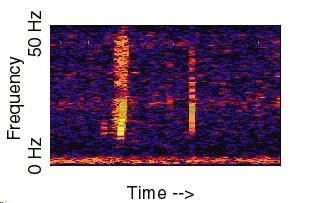
\includegraphics[width=0.5\linewidth]{images/SCP-169.jpg}
\end{figure}

尽管潜伏特工████ ████████{[}IA-1522]尽了最大的努力,这则新闻还是被泄漏给媒体,并有大量媒体进行了报道。基金会的分析结论是一个巨大的水下生物是噪音的来源,而SCP-169则被假设是噪音来源,因而从SCP-169的其他部分中发现了它的“头部”的确切位置。该声音证实了Ɣ6-0421关于SCP-169的体型异常庞大的假设。任何在未来试图确定声源位置的科学和平民团队必须以一切手段加以制止。
